\section{Hyperparameter Exploration}

\subsection{Architecture Experiment: Deeper CNN}

\subsubsection{Chosen Option}
\textbf{Option B}: Add one additional convolutional layer to the CNN architecture.

\subsubsection{Architecture Details}

The deeper CNN extends the original two-layer convolutional architecture with a third convolutional layer:

\begin{itemize}
    \item \textbf{Conv1}: 1 $\rightarrow$ 32 channels, 3$\times$3 kernel, ReLU activation
    \item \textbf{Conv2}: 32 $\rightarrow$ 64 channels, 3$\times$3 kernel, ReLU activation, MaxPool(2$\times$2)
    \item \textbf{Conv3}: 64 $\rightarrow$ 64 channels, 3$\times$3 kernel, ReLU activation, MaxPool(2$\times$2) \textit{(new layer)}
    \item \textbf{FC1}: 3,136 $\rightarrow$ 128, Dropout(0.25)
    \item \textbf{FC2}: 128 $\rightarrow$ 10 (output)
\end{itemize}

\subsubsection{Recorded Values}
\begin{itemize}
    \item Chosen option: \textbf{B - CNN Depth}
    \item Validation accuracy: \textbf{99.29\%}
    \item Number of parameters: \textbf{458,570}
    \item Training epochs: \textbf{20}
\end{itemize}

\begin{figure}[h]
    \centering
    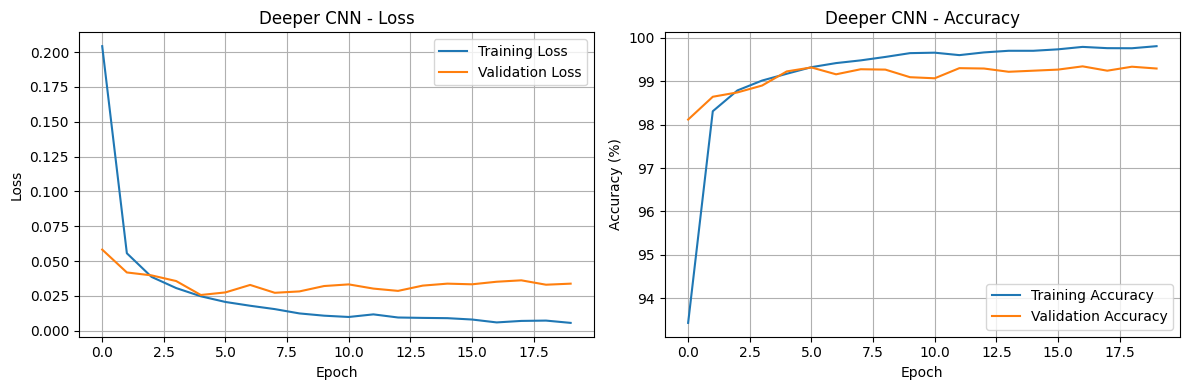
\includegraphics[width=0.8\linewidth]{section4/deeper_cnn.png}
    \caption{Training and validation curves for Deeper CNN (3 convolutional layers)}
    \label{fig:deeper-cnn}
\end{figure}

\subsubsection{Performance Analysis}

\begin{table}[h]
\centering
\begin{tabular}{|l|c|c|c|}
\hline
\textbf{Model} & \textbf{Parameters} & \textbf{Val Accuracy} & \textbf{Improvement} \\ \hline
Original CNN (2 conv layers) & 421,642 & 99.03\% & --- \\ \hline
Deeper CNN (3 conv layers)   & 458,570 & 99.29\% & +0.26\% \\ \hline
\end{tabular}
\caption{Comparison: Original CNN vs Deeper CNN}
\label{tab:deeper-cnn-comparison}
\end{table}

\textbf{Did performance improve?} 

Yes, but only marginally. The deeper CNN achieved 99.29\% validation accuracy compared to 99.03\% for the original CNN---an improvement of 0.26 percentage points. This required an additional 36,928 parameters (8.8\% increase).

The minimal improvement suggests that:
\begin{itemize}
    \item The original 2-layer CNN architecture was already near-optimal for MNIST's complexity
    \item MNIST is a relatively simple dataset that doesn't benefit significantly from deeper architectures
    \item The trade-off between added complexity and performance gain follows diminishing returns
    \item For production deployment, the simpler 2-layer CNN would be preferred due to better efficiency with comparable performance
\end{itemize}

The loss curves show that the deeper CNN maintains excellent generalization with minimal overfitting, similar to the original CNN. Both training and validation losses decrease smoothly and remain close together throughout training.

\subsection{Learning Rate Sensitivity Experiment}

\subsubsection{Experiment Setup}

To investigate the impact of learning rate on training dynamics, we trained the CNN with a learning rate 100 times larger than optimal:
\begin{itemize}
    \item \textbf{Normal learning rate}: 0.001 (Adam optimizer)
    \item \textbf{High learning rate}: 0.1 (Adam optimizer)
    \item \textbf{Training duration}: 10 epochs
\end{itemize}

\begin{figure}[h]
    \centering
    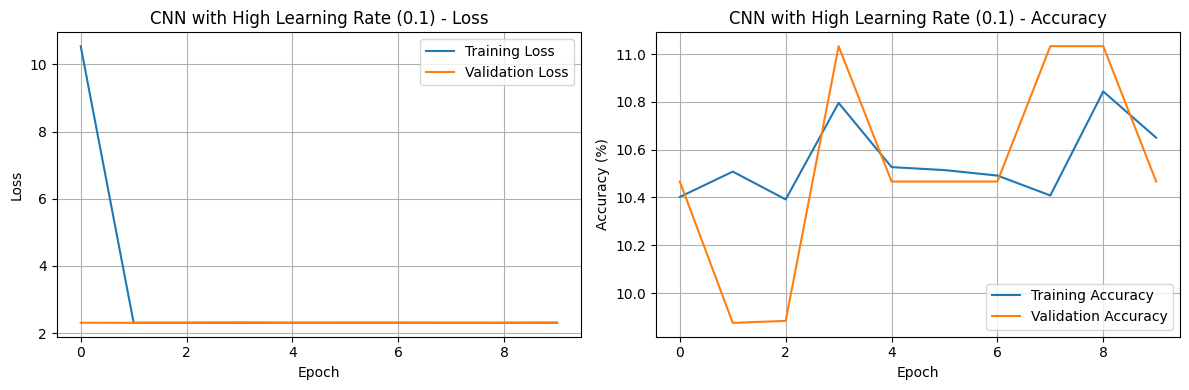
\includegraphics[width=0.8\linewidth]{section4/high_lr.png}
    \caption{Training instability with high learning rate (0.1). Note the erratic behavior and failure to converge.}
    \label{fig:high-lr}
\end{figure}

\subsubsection{Results}

\begin{table}[h]
\centering
\begin{tabular}{|l|c|c|}
\hline
\textbf{Learning Rate} & \textbf{Validation Accuracy} & \textbf{Training Loss (epoch 0)} \\ \hline
0.001 (normal)         & 99.2\%                       & 0.23                             \\ \hline
0.1 (high)             & 10.5\%                       & 10.54                            \\ \hline
\end{tabular}
\caption{Catastrophic impact of excessive learning rate}
\label{tab:learning-rate-comparison}
\end{table}

\subsubsection{Question 4.2: What happened with high learning rate? Why?}

Training with learning rate 0.1 resulted in complete failure, achieving only 10.5\% validation accuracy---barely better than random guessing for a 10-class problem (10\% baseline). The training loss remained extremely high (10.54 initially, fluctuating around 2.3) and never converged.

\textbf{Why this occurred:}

The learning rate controls the step size in gradient descent: $w_{new} = w_{old} - \alpha \cdot \nabla L$, where $\alpha$ is the learning rate. A learning rate of 0.1 is 100$\times$ larger than the optimal 0.001, causing several problems:

\begin{enumerate}
    \item \textbf{Overshooting}: The optimizer takes steps that are too large, causing it to overshoot the minimum of the loss function. Instead of converging toward optimal weights, the model bounces erratically around the loss landscape.
    
    \item \textbf{Loss landscape instability}: With such large steps, even small gradients cause massive weight updates. This prevents the model from settling into any local minimum and can cause weights to diverge to extreme values.
    
    \item \textbf{Gradient explosion}: Large learning rates can cause gradients to grow exponentially in deep networks, leading to numerical instability (though this is partially mitigated by Adam's adaptive learning rates).
    
    \item \textbf{Inability to learn features}: The dramatic weight updates prevent the convolutional filters from learning meaningful edge detectors and feature representations. The model essentially thrashes around parameter space without ever finding useful patterns in the data.
\end{enumerate}

The accuracy plot shows erratic oscillation between 9--11\%, confirming the model never learned anything beyond random guessing. The loss curves show wild fluctuations with no downward trend, characteristic of an unstable training process.

This experiment demonstrates the critical importance of proper learning rate selection. While too small a learning rate causes slow convergence, too large a learning rate---as shown here---completely prevents learning. Modern optimizers like Adam help by adapting learning rates per parameter, but cannot fully compensate for an initial learning rate that is orders of magnitude too large.

\subsection{Conclusion}

The hyperparameter exploration revealed two key insights:

\begin{enumerate}
    \item \textbf{Architectural depth}: Adding a third convolutional layer provided only marginal improvement (+0.26\%) with an 8.8\% parameter increase. For MNIST, the original 2-layer CNN appears near-optimal, and additional depth offers diminishing returns.
    
    \item \textbf{Learning rate sensitivity}: Increasing the learning rate by 100$\times$ caused catastrophic training failure, reducing accuracy from 99.2\% to 10.5\%. This demonstrates that learning rate is one of the most critical hyperparameters, and even advanced optimizers like Adam cannot compensate for grossly inappropriate values.
\end{enumerate}

These experiments illustrate fundamental principles in neural network training: model capacity should match task complexity, and optimizer hyperparameters must be carefully tuned for stable convergence.